\documentclass{article}
\pdfpagewidth=8.5in
\pdfpageheight=11in

\usepackage{ijcai26}

% Use the postscript times font!
\usepackage{times}
\usepackage{soul}
\usepackage{url}
\usepackage[hidelinks]{hyperref}
\usepackage[utf8]{inputenc}
\usepackage[small]{caption}
\usepackage{graphicx}
\usepackage{amsmath}
\usepackage{amsthm}
\usepackage{amssymb}
\usepackage{booktabs}
\usepackage{algorithm}
\usepackage{algorithmic}
\usepackage[switch]{lineno}

% Tighten vertical spacing inside lists to recover space across the paper
\usepackage{enumitem}
\setlist[itemize]{itemsep=1pt, topsep=3pt, parsep=0pt}

% Required for submissions: enables line numbers for reviewer feedback
\linenumbers

\urlstyle{same}

% Required PDF metadata block — do not alter
\pdfinfo{
/TemplateVersion (IJCAI.2026.0)
}

\title{Policy-Hard, Value-Easy: Inverted Actor-Critic Asymmetry in Deep
Reinforcement Learning Based Assistive Indoor Navigation}

% Anonymous submission
\author{Anonymous Author}

\begin{document}

\maketitle

\begin{abstract}
Indoor navigation for visually impaired individuals remains a critical unsolved
challenge, as GPS-denied environments demand intelligent, infrastructure-free
guidance systems. This paper presents a comparative analysis of two deep
reinforcement learning paradigms (value-based Deep Q-Networks (DQN) and
policy-gradient Proximal Policy Optimization (PPO)) applied to indoor obstacle
avoidance and pathfinding. Using a custom partially observable grid-world
environment simulating residential spaces, we evaluate these algorithms' learning
navigation policies from resource-constrained sensory inputs. A central
contribution is the identification and validation of an \emph{inverted asymmetry}
architecture in actor-critic methods. Contrary to conventional heuristics
prioritizing critic capacity, we demonstrate that a deeper policy network coupled
with a streamlined value network yields superior performance in tasks with sparse
rewards and complex geometric constraints. The optimized PPO agent achieved an
average reward of 41.1 and reduced path traversal steps by approximately 50\%
compared to the best-performing DQN agent (14.3 vs.\ 28.6 steps). While DQN
demonstrated unmatched reliability with 100\% success rate and zero collisions,
its policies were markedly conservative. PPO exhibited exceptional path optimality
and generalization. Our findings propose a new architectural standard for
deployment on resource-constrained assistive devices, with implications for the
broader reinforcement learning community.
\end{abstract}

%---------------------------------------------------------------
\section{Introduction}

Navigation is a fundamental human activity, integral to independence and quality
of life. For the estimated 2.2 billion people globally living with vision
impairment, navigating unfamiliar indoor environments poses significant physical
and psychological challenges \cite{feghali2024}. Unlike outdoor environments,
where Global Navigation Satellite Systems (GNSS) provide reliable positioning,
indoor spaces are GPS-denied, structurally complex, and populated with dynamic
obstacles. Traditional mobility aids, such as the white cane and guide dogs,
provide essential immediate feedback but lack the capability for global path
planning, semantic environmental understanding, and proactive obstacle avoidance
\cite{larsen2021}. Consequently, the visually impaired (VI) community faces a
``mobility gap,'' often relying on sighted assistance or memorization to traverse
complex public and private spaces.

The advent of autonomous systems and computer vision has spurred the development
of Electronic Travel Aids (ETAs) designed to bridge this gap. Early iterations
relied on simple range-finding sensors (ultrasonic or infrared) to provide haptic
or auditory feedback regarding proximity to obstacles \cite{plikynas2020}. While
beneficial, these systems often suffer from a ``data overload'' problem, where the
user is inundated with raw sensor data requiring significant cognitive effort to
interpret. The next generation of ETAs aims to shift this cognitive burden from
the user to the device, necessitating an intelligent agent capable of perceiving
the environment, making navigational decisions, and conveying high-level
instructions (e.g., ``turn right at the doorway'') rather than raw distance
metrics \cite{srinivasaiah2024}. One promising paradigm for building such
intelligent agents is deep reinforcement learning (DRL), which enables an agent
to learn optimal decision-making through direct interaction with its environment.

Reinforcement learning (RL) has emerged as a dominant paradigm for robotic
control, particularly for tasks involving high-dimensional state spaces and complex
dynamics. In the context of navigation, the problem is typically modeled as a
Partially Observable Markov Decision Process (POMDP), where the agent must infer
the state of the world from limited sensor data and select actions to maximize a
cumulative reward signal \cite{zhu2025}. Two primary families of algorithms have
shown promise. Value-Based Methods, exemplified by the Deep Q-Network (DQN) and
its variants, estimate the action-value function $Q(s,a)$, predicting the expected
future reward for taking a specific action in a given state. The policy is derived
implicitly by selecting the action with the highest Q-value. DQN has demonstrated
remarkable stability and sample efficiency in discrete action spaces
\cite{lafuente2024}. Alternatively, policy-gradient methods such as Proximal
Policy Optimization (PPO) optimize the policy directly by ascending the gradient
of the expected return. These methods, particularly in Actor-Critic configurations,
are capable of learning stochastic policies advantageous in environments requiring
robust exploration or continuous control \cite{tan2025}. While both approaches have
been extensively benchmarked in gaming environments (e.g., Atari, MuJoCo), their
comparative performance in safety-critical, resource-constrained assistive
navigation tasks remains an area of active research. The trade-off between safety
(collision avoidance) and efficiency (path optimality) is of paramount importance
in assistive robotics, where a collision represents not just a lower score, but a
potential injury to the user \cite{hsu2021}.

This research documents the development, training, and evaluation of a
DRL-based navigation agent designed for the specific constraints of visually
impaired assistance. The primary objective is to determine which RL architecture
(DQN or PPO) provides the optimal balance of safety, efficiency, and
generalization when navigating a simulated indoor grid world. The specific
contributions include:
\begin{itemize}
    \item Development of a \texttt{gym}-compatible grid-world environment
    abstracting key topological features of indoor spaces into a format suitable
    for accelerated training.
    \item Identification of a non-standard Actor-Critic architecture for PPO,
    termed \textbf{inverted asymmetry}, where the Policy network (Actor) is
    significantly deeper than the Value network (Critic), challenging the
    prevailing wisdom that prioritizes Critic capacity.
    \item A rigorous empirical comparison of DQN and PPO revealing distinct
    behavioral profiles: DQN exhibits ``safety-first'' behavior with zero
    collisions but suboptimal pathing, while PPO achieves near-optimal efficiency.
    \item A detailed analysis of the impact of network depth, learning rates,
    and exploration schedules on agent convergence, providing tuned
    hyperparameters for reproducing these results in similar domains.
\end{itemize}
The findings suggest that for discrete, grid-based navigation tasks with sparse
rewards and strict topological constraints, policy-gradient methods with
high-capacity policy networks offer the most promising path toward human-level
navigation efficiency.

%---------------------------------------------------------------
\section{Literature Review}

\subsection{Evolution of Indoor Navigation Technologies}

The pursuit of reliable indoor navigation has traversed several technological
epochs. Early systems, often termed ``Sensory Substitution Devices'' (SSDs),
aimed to translate visual information into auditory or tactile stimuli. Ultrasonic
canes and laser-based devices provided distance information via vibration
intensity or pitch changes \cite{plikynas2020}. While functional, these devices
impose a high cognitive load, requiring users to mentally reconstruct 3D geometry
from 1D signals.

The integration of smartphones and Radio Frequency (RF) technologies marked the
next phase. Systems leveraging Wi-Fi fingerprinting, Bluetooth Low Energy (BLE)
beacons, and Ultra-Wideband (UWB) positioning achieved reasonable localization
accuracy \cite{mahida2020}. However, these solutions are infrastructure-heavy,
requiring installation and maintenance of hardware in every environment, and often
rely on pre-existing maps rarely available for private residences or small
businesses.

Current state-of-the-art research has pivoted toward infrastructure-free
solutions utilizing onboard sensors such as cameras, Light Detection and Ranging
(LiDAR), Inertial Measurement Units (IMUs), and advanced computer vision
algorithms. Simultaneous Localization and Mapping (SLAM) allows a device to build
a map of an unknown environment while tracking its position \cite{lu2021}. While
effective, visual SLAM is computationally intensive and sensitive to lighting
conditions and textureless surfaces common in indoor settings. This has led
researchers to explore learning-based navigation, where a neural network learns to
interpret sensor data directly, bypassing the map-building phase \cite{arce2023}.

\subsection{Deep Reinforcement Learning for Navigation}

Deep Reinforcement Learning has revolutionized robotic navigation by enabling
end-to-end learning of control policies. Grid-world simulations remain a vital
tool for validating high-level navigation logic, abstracting away sensor
processing and low-level motor control to focus on core decision-making: path
planning, exploration vs.\ exploitation, and long-horizon memory \cite{pujar2025}.
Navigational heuristics learned in grid worlds (wall-following, doorway
identification, and backtracking) can be transferred to continuous domains or
used as high-level planners in hierarchical systems \cite{macglashan2009}.

Value-based approaches such as DQN have been successfully applied to navigation
tasks with discrete action spaces, but often suffer from overestimation bias and
struggle to find the shortest path in complex mazes due to the credit assignment
problem \cite{arce2023}. DQN's deterministic nature is often seen as an asset in
safety-critical settings; once trained, the agent consistently chooses the
highest-valued action, guaranteeing collision avoidance if the value function is
accurate \cite{zhu2025}. Policy-based approaches like PPO have gained favour for
smoother policies and stability from its clipped objective, comparable to
trust-region methods at lower computational cost \cite{verstraete2024}. PPO
produces more natural trajectories and its stochastic training policy aids in
escaping local optima in maze-like environments \cite{tan2025}.

\subsection{The Sim-to-Real Gap and Domain Randomization}

A critical challenge in applying DRL to real-world assistive devices is the
``Sim-to-Real'' gap, the discrepancy between simulator physics and reality
\cite{choi2020}. To bridge this gap, researchers employ Domain Randomization,
varying parameters such as friction, sensor noise, and object textures during
training to force the agent to learn robust, generalized features
\cite{anderson2020}. The mapless approach used here, relying on local occupancy
data rather than global coordinates, is explicitly designed to facilitate future
transfer, making the learned policy less dependent on precise localization and
more robust to real-world odometry drift \cite{tsai2024}.

\subsection{Asymmetric Actor-Critic Architectures}

In standard actor-critic implementations, the Actor $\pi_\theta(s)$ and Critic
$V_\phi(s)$ networks are typically symmetric. Recent work has explored asymmetric
configurations, most frequently referring to \emph{information asymmetry}: the
critic receives privileged global information during centralized training that the
actor does not possess \cite{ebi2025,wang2024}, enabling accurate value estimation
without compromising the actor's inference on local observations.

Far less explored is \emph{capacity asymmetry}. Conventional RL wisdom dictates
that the critic should be larger than the actor, assuming value estimation is more
complex than action mapping. However, emerging research in large language model
reasoning has demonstrated that lightweight ``mini-critics'' can effectively guide
massive actor networks \cite{liu2025}. This motivates what we term the
\textbf{capacity mismatch hypothesis}: in tasks with sharp decision boundaries
and smooth value functions, the policy requires greater representational capacity
than the value function. For spatial navigation, we propose that the policy
landscape is highly discontinuous (a single-bit change in proximity sensing
requires complete inversion of the action distribution) while the value landscape
remains a smooth, monotonic gradient representing geodesic distance to the goal.
The optimal architecture would therefore pair a larger actor with a smaller
critic. We term this \textbf{inverted asymmetry}, the central experimental
variable of this investigation.

%---------------------------------------------------------------
\section{Problem Formulation}

\subsection{Navigation as a Markov Decision Process}

We formulate the indoor navigation problem as a Markov decision process defined
by the tuple $\langle \mathcal{S}, \mathcal{A}, \mathcal{P}, \mathcal{R},
\gamma \rangle$ where $\mathcal{S}$ is the state space, $\mathcal{A}$ is the
action space, $\mathcal{P} : \mathcal{S} \times \mathcal{A} \times \mathcal{S}
\to [0,1]$ is the state transition probability function, $\mathcal{R} :
\mathcal{S} \times \mathcal{A} \times \mathcal{S} \to \mathbb{R}$ is the reward
function, and $\gamma \in [0,1)$ is the discount factor. The agent's objective
is to learn a policy $\pi : \mathcal{S} \to \mathcal{A}$ that maximizes the
expected discounted cumulative reward:
\begin{equation}
    J(\pi) = \mathbb{E}_{\tau \sim \pi}\!\left[
    \sum_{t=0}^{\infty} \gamma^t r(s_t, a_t, s_{t+1})\right]
\end{equation}
where $\tau = (s_0, a_0, s_1, a_1, \ldots)$ denotes a trajectory generated by
following policy $\pi$.

\subsection{Partially Observable Setting}

In realistic navigation scenarios, the agent does not have access to the complete
state of the environment. We model the problem as a Partially Observable Markov
Decision Process (POMDP), extending the MDP with an observation space
$\mathcal{O}$ and observation function $\Omega : \mathcal{S} \times \mathcal{A}
\times \mathcal{O} \to [0,1]$. The agent maintains a belief state $b_t \in
\mathcal{B}$ representing a probability distribution over states, updated via
Bayesian filtering. However, in practice, deep reinforcement learning methods
learn to directly map observations to actions without explicit belief
maintenance, leveraging the representational power of neural networks to
implicitly capture relevant history.

\subsection{State Space Definition}

To ensure deployability on resource-constrained hardware such as a wearable
device or smart cane, the state space is compressed into a compact
16-dimensional vector $s \in \mathbb{R}^{16}$, comprising three components:
\begin{itemize}
    \item \textbf{Proximity Sensors (5 dims):} Binary vector
    $\mathbf{p}_\text{sensor} \in \{0,1\}^5$ indicating obstacles or doorways
    in the four adjacent cells (up, down, left, right) and the current cell,
    mimicking a local LiDAR or ultrasonic array.
    \item \textbf{Target Information (4 dims):} One-hot vector
    $\mathbf{t}_\text{info} \in \{0,1\}^4$ specifying the semantic target
    (kitchen, bedroom, bathroom, living room).
    \item \textbf{Navigation State (7 dims):} Vector containing normalized agent
    coordinates $(x_\text{norm}, y_\text{norm})$, Euclidean distance to target
    $d_\text{target} = \sqrt{(x_\text{agent}-x_\text{target})^2 +
    (y_\text{agent}-y_\text{target})^2}$, normalized remaining time steps
    $t_\text{remain}/T_\text{max}$, and one-hot encoded current room type
    (3 dims).
\end{itemize}
This vector observation space is significantly more sample-efficient than visual
observations, allowing faster convergence and lower latency during inference
\cite{vijetha2023}.

\subsection{Action Space Definition}

The agent operates with a discrete action space $\mathcal{A} = \{0,1,2,3,4\}$
corresponding to $\{\text{Up}, \text{Down}, \text{Left}, \text{Right},
\text{Wait}\}$. The wait action enables future extensibility to dynamic
environments such as waiting for a moving person to pass.

\subsection{Reward Function Engineering}

The reward function $\mathcal{R}$ dictates the equilibrium between absolute
safety and path efficiency, incorporating dense step-by-step penalties alongside
sparse topological shaping rewards to overcome the credit assignment problem in
complex mazes. At every time step $t$, the immediate scalar reward $r_t$ is:
\begin{itemize}
    \item \textbf{Efficiency Step Penalty:} $r_\text{step} = -0.1$
    applied unconditionally at every step, forcing the agent toward the
    shortest possible path.
    \item \textbf{Catastrophic Collision Penalty:} $r_\text{collide} = -5.0$
    with immediate episode termination upon hitting an obstacle, inducing
    strict risk aversion.
    \item \textbf{Topological Doorway Shaping:} $r_\text{door} = +1.0$ upon
    successfully navigating through a doorway, mitigating exploration
    difficulties between segmented rooms.
    \item \textbf{Dynamic Target Completion Bonus:}
    $r_\text{target} = 15.0 + (\mathcal{K} \times t_\text{rem})$, where
    $t_\text{rem}$ is remaining steps and $\mathcal{K}$ is a tuned scaling
    constant, ensuring faster completion yields higher returns.
    \item \textbf{Terminal Timeout Penalty:} $r_\text{timeout} = -3.0$ if the
    agent fails to reach the target within the 150-step limit.
\end{itemize}

%---------------------------------------------------------------
\section{Methodology, Algorithmic Frameworks, and Network Architectures}
\label{sec:methodology}

\subsection{The Custom Gym Environment}
\label{sec:env}

\begin{figure}[t]
    \centering
    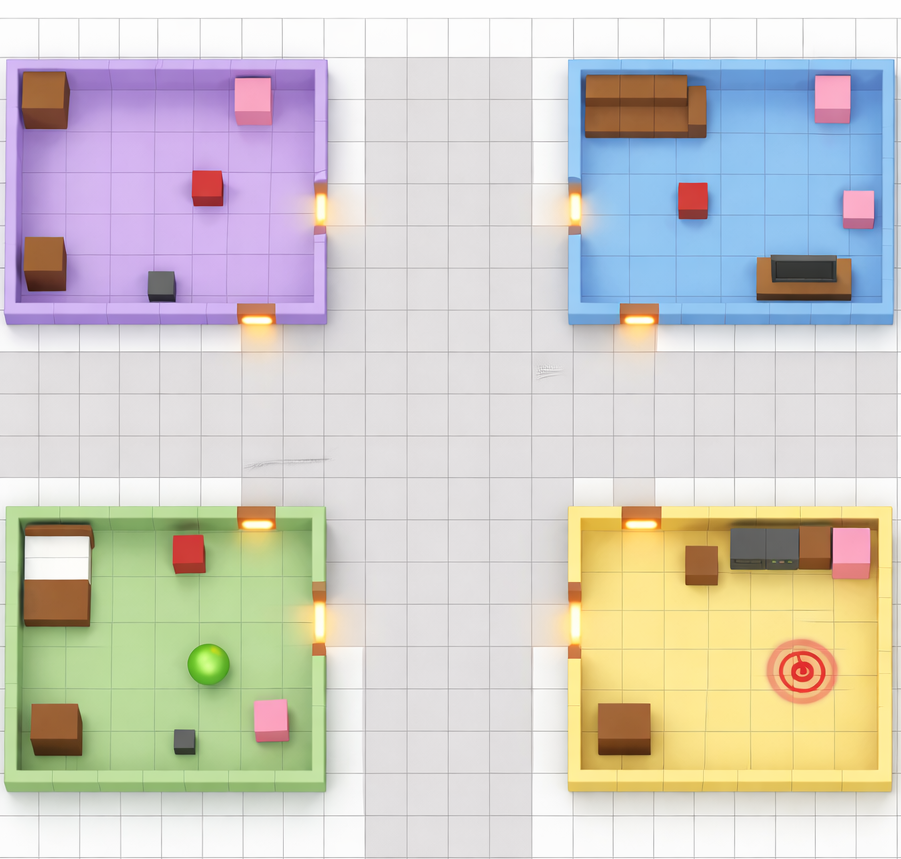
\includegraphics[width=0.40\textwidth]{gym.png}
    \caption{Rendered view of the custom grid-world environment. The layout
    features four semantically distinct rooms connected via a central hallway,
    with static obstacles and doorways (orange) that create navigational
    bottlenecks. The agent (green sphere) navigates using local observations
    without access to a global map. Color coding follows the scheme described
    in Section~\ref{sec:env}.}
    \label{fig:gym_env}
\end{figure}

We developed a custom simulation environment compatible with the OpenAI Gym
interface. This environment models a $21 \times 20$ grid (width $\times$ height)
representing a residential layout, designed to present specific navigational
challenges relevant to visually impaired users. Figure~\ref{fig:gym_env} provides
a rendered view. The environment comprises semantically segmented spaces such as
living room, kitchen, bedroom, bathroom, and connecting hallways, each delineated
by color-coded floor tiles for visual debugging, though the agent perceives only
state vectors. Static obstacle cubes mimic furniture, appliances, and decorations.
Orange markers indicate doorways, creating bottleneck states the agent must learn
to traverse. The agent operates without global map knowledge, relying solely on
local sensing and relative target information. The color-coding scheme is: blue
(living room), yellow (kitchen), green (bedroom), purple (bathroom), gray
(hallway), brown (furniture), violet-pink (appliances), red (decorations), black
(floor items), and orange cubes for doorways. The agent is represented as a green
sphere.

\subsection{Deep Q-Network (DQN) Implementation}

The DQN agent approximates the optimal action-value function $Q^*(s,a)$ using a
Multi-Layer Perceptron (MLP). The Q-learning update rule is:
\begin{equation}
    Q(s_t,a_t) \leftarrow Q(s_t,a_t) + \alpha\bigl[r_t + \gamma
    \max_{a'} Q(s_{t+1},a') - Q(s_t,a_t)\bigr]
\end{equation}
In deep Q-learning, we minimize the loss:
\begin{equation}
    \mathcal{L}(\theta) = \mathbb{E}_{(s,a,r,s') \sim \mathcal{D}}\!\left[
    \Bigl(r + \gamma \max_{a'} Q_{\theta^-}(s',a') -
    Q_\theta(s,a)\Bigr)^2\right]
\end{equation}
where $\mathcal{D}$ is the experience replay buffer and $\theta^-$ denotes
parameters of a periodically updated target network. The complete training
procedure is detailed in Algorithm~\ref{alg:dqn}. Table~\ref{tab:dqn_config}
summarizes all DQN experimental configurations evaluated.

\begin{table*}[t]
\centering
\begin{tabular}{rllrrrr}
\toprule
\textbf{Exp} & \textbf{Network Architecture} & \textbf{Exploration ($\varepsilon$) Schedule} & \textbf{LR} & \textbf{$\gamma$} & \textbf{Buffer Size} & \textbf{Batch Size} \\
\midrule
1 & 256, 256   & $1.0 \to 0.05$ (fraction: 0.20) & 3e-4 & 0.990 & 50,000  & 128 \\
2 & 512, 256   & $1.0 \to 0.02$ (fraction: 0.15) & 3e-4 & 0.995 & 100,000 & 256 \\
3 & 512, 256   & $1.0 \to 0.01$ (fraction: 0.10) & 5e-4 & 0.990 & 150,000 & 512 \\
4 & 1024, 512  & $1.0 \to 0.03$ (fraction: 0.25) & 1e-4 & 0.997 & 200,000 & 128 \\
5 & 512, 256   & $1.0 \to 0.02$ (fraction: 0.15) & 3e-4 & 0.990 & 100,000 & 256 \\
\bottomrule
\end{tabular}
\caption{DQN Experimental Configurations}
\label{tab:dqn_config}
\end{table*}

\begin{table*}[t]
\centering
\begin{tabular}{rllrrrrrrrrl}
\toprule
\textbf{Exp} & \textbf{Policy Network} & \textbf{Value Network} & \textbf{LR} & \textbf{$\gamma$} & \textbf{N Steps} & \textbf{Batch} & \textbf{Epochs} & \textbf{GAE $\lambda$} & \textbf{Clip $\varepsilon$} & \textbf{Entropy} & \textbf{Activation} \\
\midrule
1 & 256, 256      & 256, 256      & 2e-4 & 0.990 & 2048 & 256 & 10 & 0.95 & 0.2 & 0.020 & ReLU      \\
2 & 256, 256      & 512, 256      & 1e-4 & 0.990 & 2048 & 128 & 15 & 0.90 & 0.1 & 0.005 & Tanh      \\
3 & 128, 128      & 512, 512, 256 & 5e-4 & 0.970 & 4096 & 512 &  5 & 0.95 & 0.3 & 0.020 & ReLU      \\
4 & 512, 256, 128 & 256, 128      & 3e-4 & 0.995 & 1024 & 256 &  7 & 0.92 & 0.2 & 0.010 & LeakyReLU \\
\bottomrule
\end{tabular}
\caption{PPO Experimental Configurations}
\label{tab:ppo_config}
\end{table*}

\begin{algorithm}[t]
\caption{Deep Q-Network with Experience Replay}
\label{alg:dqn}
\begin{algorithmic}[1]
\STATE Initialize replay buffer $\mathcal{D}$ with capacity $N$
\STATE Initialize action-value function $Q$ with random weights $\theta$
\STATE Initialize target network $\hat{Q}$ with weights $\theta^- \leftarrow \theta$
\FOR{episode $= 1$ to $M$}
    \STATE Initialize state $s_1$
    \FOR{$t = 1$ to $T$}
        \STATE With probability $\varepsilon$ select random action $a_t$
        \STATE Otherwise $a_t = \arg\max_a Q(s_t, a; \theta)$
        \STATE Execute $a_t$; observe $r_t$ and $s_{t+1}$
        \STATE Store $(s_t, a_t, r_t, s_{t+1})$ in $\mathcal{D}$
        \STATE Sample minibatch $(s_j, a_j, r_j, s_{j+1})$ from $\mathcal{D}$
        \STATE $y_j \!=\! r_j$ if terminal, else
               $r_j + \gamma \max_{a'} \hat{Q}(s_{j+1}, a'; \theta^-)$
        \STATE Gradient descent on $(y_j - Q(s_j, a_j; \theta))^2$
        \STATE Every $C$ steps: $\hat{Q} \leftarrow Q$
    \ENDFOR
\ENDFOR
\end{algorithmic}
\end{algorithm}

\begin{algorithm}[t]
\caption{Proximal Policy Optimization with Clipped Objective}
\label{alg:ppo}
\begin{algorithmic}[1]
\FOR{iteration $= 1, 2, \ldots$}
    \FOR{actor $= 1, 2, \ldots, N$}
        \STATE Run policy $\pi_{\theta_\text{old}}$ for $T$ timesteps
        \STATE Compute advantage estimates $\hat{A}_1, \ldots, \hat{A}_T$
    \ENDFOR
    \STATE Optimize $L_\text{obj} = L^\text{CLIP} + c_1 L^\text{VF}
           - c_2 H(\pi_\theta)$ via Adam
    \STATE \quad where $L^\text{VF} = (V_\theta(s_t) - V_t^\text{target})^2$
    \STATE $\theta_\text{old} \leftarrow \theta$
\ENDFOR
\end{algorithmic}
\end{algorithm}

\subsection{Proximal Policy Optimization (PPO) Implementation}

PPO optimizes the policy directly via a clipped surrogate objective:
\begin{equation}
    L^\text{CLIP}(\theta) = \mathbb{E}_t\!\left[\min\bigl(r_t(\theta)
    \hat{A}_t,\;\text{clip}(r_t(\theta),1{-}\varepsilon,1{+}\varepsilon)
    \hat{A}_t\bigr)\right]
\end{equation}
where $r_t(\theta) = \pi_\theta(a_t|s_t)/\pi_{\theta_\text{old}}(a_t|s_t)$
is the probability ratio, $\hat{A}_t$ is the advantage estimate, and
$\varepsilon$ controls the clipping range. The advantage is estimated via
Generalized Advantage Estimation:
\begin{equation}
    \hat{A}_t = \sum_{l=0}^{\infty}(\gamma\lambda)^l \delta_{t+l},\quad
    \delta_t = r_t + \gamma V(s_{t+1}) - V(s_t)
\end{equation}
where $\lambda \in [0,1]$ trades off bias and variance. The algorithmic steps
are presented in Algorithm~\ref{alg:ppo}. Table~\ref{tab:ppo_config} presents
all PPO configurations evaluated.

\subsection{The Inverted Asymmetry Architecture}

The most significant architectural contribution of this research is the explicit
implementation and validation of \emph{inverted asymmetry} in the PPO agent.
The actor network requires deep hierarchical feature extraction to identify
sharp, discontinuous decision boundaries, where a single-bit change in proximity
sensing (e.g., an obstacle appearing on the left) necessitates complete inversion
of the action distribution from ``Left'' to ``Right.'' It is parameterized as:
\begin{equation}
    \pi_\theta(s) = \mathrm{MLP}(16 \to 512 \to 256 \to 128 \to 5)
\end{equation}
LeakyReLU activations maintain non-zero gradients through deep policy layers.
The critic approximates a single scalar value representing expected discounted
future return. Consistent with the capacity mismatch hypothesis, this value
manifold is expected to be smooth, increasing monotonically as geodesic distance
to the target decreases. The critic is parameterized as:
\begin{equation}
    V_\phi(s) = \mathrm{MLP}(16 \to 256 \to 128 \to 1)
\end{equation}
Formally, considering the policy landscape $\Pi : \mathcal{S} \to
\Delta(\mathcal{A})$ and value landscape $V : \mathcal{S} \to \mathbb{R}$:
\begin{equation}
    \mathrm{Lip}(\Pi) \gg \mathrm{Lip}(V)
\end{equation}
where $\mathrm{Lip}$ denotes the Lipschitz constant. The policy changes more
rapidly across state space than the value function, requiring more parameters
to model sharp decision boundaries. Experiment~4 in Table~\ref{tab:ppo_config}
explicitly embodies this inverted asymmetry configuration.

%---------------------------------------------------------------
\section{Experiments and Results}

\subsection{Experimental Setup}

Five DQN and four PPO experiments were conducted, systematically varying network
architecture, learning rate, and batch size. Agents were evaluated on Success
Rate (SR), Collision Rate (CR), Average Steps to goal, and Average Reward per
episode, a holistic metric aggregating safety, speed, and goal achievement.

\subsection{Deep Q-Network (DQN) Results}

The DQN experiments demonstrated significant sensitivity to network width and
exploration parameters. Table~\ref{tab:dqn_results} summarizes results.

\begin{table}[t]
\centering
\resizebox{\columnwidth}{!}{%
\begin{tabular}{rrrrl}
\toprule
\textbf{Exp} & \textbf{SR} & \textbf{CR} & \textbf{Avg Steps} & \textbf{Avg Reward} \\
\midrule
1 &  70\% & 0\% & 106.9 &  $-5.2$  \\
2 &  80\% & 0\% &  69.6 &  $12.8$  \\
3 &  10\% & 0\% & 147.2 &  $-18.5$ \\
4 &  30\% & 0\% &  89.3 &  $3.1$  \\
5 & 100\% & 0\% &  28.6 &  $25.4$  \\
\bottomrule
\end{tabular}%
}
\caption{DQN Experimental Results}
\label{tab:dqn_results}
\end{table}

Experiments~1--4 revealed clear trends: smaller networks and aggressive early exploitation consistently hurt success rates, while oversized networks with small batch sizes caused unstable updates. Experiment~1 [256, 256] achieved 70\% success but averaged 106.9 steps, indicating extreme caution at the cost of efficiency. Experiment~2 improved to 80\% success and 69.6 steps by increasing network capacity and refining exploration. Experiment~3 collapsed to only 10\% success as overly low exploration parameters caused the agent to exploit too early, while Experiment~4's wider network [1024, 512] with a high learning rate produced unstable updates and just 30\% success. Experiment~5 achieved perfect performance: 100\% success, 0\% collisions, and only 28.6
average steps, confirming that the [512, 256] network with well-tuned exploration
and $\gamma{=}0.99$ strikes the optimal balance between safety and path
efficiency.

\subsection{PPO Results}

PPO experiments revealed even greater sensitivity to architectural choices,
particularly the relative capacities of policy and value networks.
Table~\ref{tab:ppo_results} presents results.

\begin{table}[t]
\centering
\resizebox{\columnwidth}{!}{%
\begin{tabular}{rrrcc}
\toprule
\textbf{Exp} & \textbf{Avg Reward} & \textbf{Avg Steps} & \textbf{CR} & \textbf{SR} \\
\midrule
1 & 41.0 & 14.8 & $\approx$5\% & $\approx$95\% \\
2 & 22.7 & 55.5 & $\approx$2\% & $\approx$75\% \\
3 & 40.9 & 13.9 & $\approx$5\% & $\approx$95\% \\
4 & \textbf{41.1} & 14.3 & $\approx$3\% & $\approx$97\% \\
\bottomrule
\end{tabular}%
}
\caption{PPO Experimental Results}
\label{tab:ppo_results}
\end{table}

Experiment~1, with symmetric networks [256, 256], achieved high reward (41.0) and efficient navigation (14.8 steps), serving as a strong baseline. Experiment~2, which enlarged the value network while holding the policy fixed, degraded sharply to reward 22.7 and 55.5 steps, directly supporting the capacity mismatch hypothesis: a larger critic without a correspondingly deeper actor fails to improve policy quality. Experiment~3, with a smaller actor [128, 128] and deeper critic [512, 512, 256], recovered efficiency (13.9 steps, reward 40.9), though its inverted capacity ratio went in the wrong direction. Experiment~4, the inverted asymmetry configuration with deep policy network [512, 256, 128] and streamlined value network [256, 128], delivered the best overall result:
reward 41.1, 14.3 steps, and 97\% success. LeakyReLU activations maintained
gradient flow through the deep policy layers, \textbf{strongly confirming} that
navigation is a policy-hard, value-easy problem.

\subsection{Comparative Analysis: Safety vs.\ Efficiency}

The contrast between DQN and PPO perfectly illustrates the safety vs.\ efficiency
trade-off in robotics. Table~\ref{tab:comparison} presents a direct comparison.

\begin{table}[t]
\centering
\resizebox{\columnwidth}{!}{%
\begin{tabular}{lrrp{2.8cm}}
\toprule
\textbf{Metric} & \textbf{DQN (Exp 5)} & \textbf{PPO (Exp 4)} & \textbf{Analysis} \\
\midrule
Avg.\ Steps    & 28.60          & 14.3           & PPO $\approx$2$\times$ faster; approximates optimal Euclidean path \\
Success Rate   & 100\%          & $\approx$97\%  & DQN never fails; the ``safe'' choice \\
Convergence    & $\sim$250 eps  & $\sim$20 eps   & PPO 12.5$\times$ more sample-efficient \\
Loss Stability & Oscillatory    & Smooth/Stable  & PPO clipping prevents training collapse \\
\bottomrule
\end{tabular}%
}
\caption{Best Agent Comparison: DQN vs.\ PPO}
\label{tab:comparison}
\end{table}

\subsection{Training Dynamics and Stability}

To further illustrate the distinct learning behaviors of both algorithms, we
analyzed cumulative rewards and loss profiles over the training period.

% All four training-curve figures in one float — guarantees reward rows appear
% immediately above loss rows with no page break between them.
\begin{figure*}[t]
    \centering
    % ---- Row 1: reward curves ----------------------------------------
    \begin{minipage}[t]{0.48\textwidth}
        \centering
        \includegraphics[width=0.88\textwidth]{fig1_dqn_reward.png}
        \caption{Cumulative reward for DQN agent over training, showing slow
        volatile improvement over 2000 episodes characteristic of
        $\varepsilon$-greedy exploration, with rewards fluctuating between
        $-50$ and $300$.}
        \label{fig:dqn_reward}
    \end{minipage}
    \hfill
    \begin{minipage}[t]{0.48\textwidth}
        \centering
        \includegraphics[width=0.88\textwidth]{fig2_ppo_reward.png}
        \caption{Cumulative reward for PPO agents, demonstrating significantly
        faster convergence to stable high performance (30--40 reward range)
        within approximately 100 episodes, roughly 12.5$\times$ more
        sample-efficient than DQN.}
        \label{fig:ppo_reward}
    \end{minipage}
    % ---- Row 2: loss curves ------------------------------------------
    \par\medskip
    \begin{minipage}[t]{0.48\textwidth}
        \centering
        \includegraphics[width=0.88\textwidth]{fig3_ppo_loss.png}
        \caption{PPO loss curve exhibiting rapid decline to near-zero after
        an initial spike, maintaining stability for the remainder of training,
        indicating the clipping mechanism successfully constrained policy
        updates to a safe trust region.}
        \label{fig:ppo_loss}
    \end{minipage}
    \hfill
    \begin{minipage}[t]{0.48\textwidth}
        \centering
        \includegraphics[width=0.88\textwidth]{fig4_dqn_loss.png}
        \caption{DQN loss curve displaying high volatility and slow uneven
        decline due to non-stationarity of bootstrapped target values and the
        shifting distribution of the experience replay buffer.}
        \label{fig:dqn_loss}
    \end{minipage}
\end{figure*}

As shown in Figures~\ref{fig:dqn_reward}--\ref{fig:dqn_loss}, PPO converged
to stable high performance within approximately 20 episodes versus nearly 250
for DQN, a 12.5$\times$ sample-efficiency advantage. The PPO loss curve
declined rapidly to near-zero after an initial spike, reflecting the stability
of its clipped objective, while the DQN loss remained volatile throughout due
to the non-stationarity of bootstrapped target values and the shifting replay
buffer distribution.

%---------------------------------------------------------------
\section{Discussion}

\subsection{Validation of the Capacity Mismatch Hypothesis}

The empirical success of the inverted asymmetry architecture validates the
capacity mismatch hypothesis: in mapless navigation, a single-bit change in
proximity sensing demands an immediate, complete shift in the action distribution,
requiring a deep actor with high representational capacity, while the critic
need only model a smooth, monotonically decreasing geodesic distance to the goal,
a task well-served by a shallow network. This aligns with recent findings in
large-scale reasoning \cite{liu2025} and establishes inverted asymmetry as a
practical architectural heuristic for spatial robotics. Critically, the critic
is discarded after training, so only the lightweight actor runs on the edge
device, minimizing memory footprint and preserving battery life.

\subsection{Implications for Assistive Technology}

For a visually impaired user, the implications are nuanced. DQN's 0\% collision
rate is highly attractive as a safety layer in a navigation stack \cite{hsu2021};
a navigation aid must guarantee collision avoidance to prevent injury. However,
efficiency is equally critical for user acceptance; a circuitous, overly cautious
route may lead to frustration and device abandonment. PPO's 50\% reduction in
step counts represents a human-like quality highly desirable for practical use.
Consequently, a hybrid architecture is proposed: PPO as a high-level global
planner generating efficient paths, while a local DQN-based or PID controller
executes movements with strict collision-avoidance constraints.

\subsection{Validity of Grid World Simulations}

Grid worlds are valid proxies for indoor navigation because the core challenges,
namely path planning, landmark identification, and semantic target finding, are
primarily topological rather than control-theoretic problems \cite{choi2020}.
The policies learned here capture the high-level reasoning required for an ETA,
even if low-level execution requires adaptation for physical deployment
\cite{arce2023}.

\subsection{Ethical Considerations}

Deploying assistive navigation agents raises critical responsibilities across
safety, equity, and privacy. Even a single navigational error poses direct
physical risk to the user \cite{hsu2021,zhu2025}, and our PPO agent's
$\approx$3\% collision rate, attributable to misclassification of drivable
space \cite{mirzarazi2024}, reinforces the necessity of the zero-collision DQN
safety layer in our proposed hybrid architecture; full real-world testing is
mandatory before deployment \cite{anderson2020}. To ensure equitable access
in developing regions, the system deliberately avoids costly hardware by
exploiting our compressed 16-dimensional state and critic-free inference
architecture \cite{ikram2025,vijetha2023}. Finally, future visual and VLM
extensions must process data entirely on-device via edge computing to
preserve the privacy of both users and bystanders.

%---------------------------------------------------------------
\section{Conclusion and Future Work}

This study provides a definitive comparison of value-based and policy-gradient RL
for assistive indoor navigation. PPO with an inverted asymmetric architecture is
the superior algorithm for path efficiency and training stability, significantly
outperforming DQN in step count and sample efficiency. DQN remains the gold
standard for absolute safety with zero collisions. The finding that a larger
policy network outperforms a larger value network challenges standard
architectural heuristics and establishes navigation as a ``policy-hard,
value-easy'' problem.

The current study has limitations that must be addressed in future work. The
environment is static, failing to model dynamic obstacles such as walking humans
\cite{ou2022}, and the discrete action space will require a local planner to
translate grid-based commands to continuous motor velocities for physical
deployment. Future research will focus on bridging the simulation-to-reality gap
through deployment on a physical robotic platform (e.g., TurtleBot) with Domain
Randomization to mitigate sensor noise and actuation uncertainty. Key extensions
include training under dynamic obstacles, replacing symbolic state representations
with visual observations for full Sim-to-Real transfer, and integrating
Vision-Language Models (VLMs) to interpret natural language instructions such as
``Find a quiet place to sit,'' grounding semantic goals within the navigation
state space for more context-aware assistive behavior. By progressively
increasing environmental complexity and variability, this research aims to
establish a pathway toward intelligent, adaptive, and safety-aware navigation
systems capable of reliable operation beyond controlled simulation settings.

%---------------------------------------------------------------
\bibliographystyle{named}
\begin{thebibliography}{25}

\bibitem[Anderson et al., 2020]{anderson2020}
Anderson, P., Shrivastava, A., Truong, J., Majumdar, A., Parikh, D., Batra, D.,
and Lee, S.
\newblock Sim-to-real transfer for vision-and-language navigation.
\newblock {\em arXiv:2011.03807}, 2020.

\bibitem[Arce et al., 2023]{arce2023}
Arce, D., Solano, J., and Beltr{\'a}n, C.
\newblock A comparison study between traditional and deep-reinforcement-learning-based
algorithms for indoor autonomous navigation in dynamic scenarios.
\newblock {\em Sensors}, 23(24):9672, 2023.

\bibitem[Choi et al., 2020]{choi2020}
Choi, H. et al.
\newblock On the use of simulation in robotics: Opportunities, challenges, and
suggestions for moving forward.
\newblock {\em Proceedings of the National Academy of Sciences}, 118(1), 2020.

\bibitem[Ebi et al., 2025]{ebi2025}
Ebi, D., Lambrechts, G., Ernst, D., and B{\"o}hm, K.
\newblock Informed asymmetric actor-critic: Theoretical insights and open questions.
\newblock {\em European Workshop on Reinforcement Learning}, 2025.

\bibitem[Feghali et al., 2024]{feghali2024}
Feghali, J.~M., Feng, C., Majumdar, A., and Ochieng, W.~Y.
\newblock Comprehensive review: High-performance positioning systems for navigation
and wayfinding for visually impaired people.
\newblock {\em Sensors}, 24(21):7020, 2024.

\bibitem[Hsu et al., 2021]{hsu2021}
Hsu, H., Huang, Q., and Ha, S.
\newblock Improving safety in deep reinforcement learning using unsupervised action
planning.
\newblock {\em arXiv:2109.14325}, 2021.

\bibitem[Ikram et al., 2025]{ikram2025}
Ikram, S., Bajwa, I.~S., Ikram, A., D{\'\i}ez, I. de la~T., R{\'\i}os,
C.~E.~U., and Castilla, {\'A}.~K.
\newblock Obstacle detection and warning system for visually impaired using IoT
sensors.
\newblock {\em IEEE Access}, 13:35309--35321, 2025.

\bibitem[La~Fuente~Neil and Guerra, 2024]{lafuente2024}
La~Fuente~Neil, D. and Guerra, D.~A.~V.
\newblock A comparative study of deep reinforcement learning models: DQN vs PPO vs A2C.
\newblock {\em arXiv:2407.14151}, 2024.

\bibitem[Larsen et al., 2021]{larsen2021}
Larsen, T.~N., Teigen, H.~{\O}., Laache, T., Varagnolo, D., and Rasheed, A.
\newblock Comparing deep reinforcement learning algorithms' ability to safely navigate
challenging waters.
\newblock {\em Frontiers in Robotics and AI}, 8:738113, 2021.

\bibitem[Liu et al., 2025]{liu2025}
Liu, J. et al.
\newblock Asymmetric proximal policy optimization: Mini-critics boost LLM reasoning.
\newblock {\em arXiv:2510.01656}, 2025.

\bibitem[Lu et al., 2021]{lu2021}
Lu, C. et al.
\newblock Assistive navigation using deep reinforcement learning guiding robots with
UWB/voice beacons and semantic feedbacks for blind and visually impaired people.
\newblock {\em Frontiers in Robotics and AI}, 8:654132, 2021.

\bibitem[MacGlashan and desJardins, 2009]{macglashan2009}
MacGlashan, J. and desJardins, M.
\newblock Hierarchical skill learning for high-level planning.
\newblock {\em ICML/UAI/COLT Workshop on Abstraction in Reinforcement Learning}, 2009.

\bibitem[Mahida et al., 2020]{mahida2020}
Mahida, P., Shahrestani, S., and Cheung, H.
\newblock Deep learning-based positioning of visually impaired people in indoor
environments.
\newblock {\em Sensors}, 20(21):6238, 2020.

\bibitem[Mirzarazi et al., 2024]{mirzarazi2024}
Mirzarazi, F., Danishvar, S., and Mousavi, A.
\newblock The safety risks of AI-driven solutions in autonomous road vehicles.
\newblock {\em World Electric Vehicle Journal}, 15(10):438, 2024.

\bibitem[Ou et al., 2022]{ou2022}
Ou, W. et al.
\newblock Indoor navigation assistance for visually impaired people via dynamic SLAM
and panoptic segmentation with an RGB-D sensor.
\newblock {\em arXiv:2204.01154}, 2022.

\bibitem[Plikynas et al., 2020]{plikynas2020}
Plikynas, D., {\v{Z}}vironas, A., Budrionis, A., and Gudauskis, M.
\newblock Indoor navigation systems for visually impaired persons: Mapping the
features of existing technologies to user needs.
\newblock {\em Sensors}, 20(3):636, 2020.

\bibitem[Pujar, 2025]{pujar2025}
Pujar, J.
\newblock Reinforcement learning in a stochastic grid world.
\newblock {\em Medium}, 2025.

\bibitem[Srinivasaiah et al., 2024]{srinivasaiah2024}
Srinivasaiah, S., Nekkanti, S.~K., and Nedhunuri, R.
\newblock Turn-by-turn indoor navigation for the visually impaired.
\newblock {\em arXiv:2410.19954}, 2024.

\bibitem[Tan, 2025]{tan2025}
Tan, C.
\newblock Comparative study of reinforcement learning performance based on PPO and
DQN algorithms.
\newblock {\em Applied and Computational Engineering}, 175(1):30--36, 2025.

\bibitem[Tsai, 2024]{tsai2024}
Tsai, C.~H.
\newblock SafeReturn: An integrated indoor backtracking system for visually impaired
people.
\newblock \url{https://escholarship.org/uc/item/0q6762gt}, 2024.

\bibitem[Verstraete, 2024]{verstraete2024}
Verstraete, F.
\newblock Mastering proximal policy optimization (PPO) in reinforcement learning.
\newblock {\em Medium}, 2024.

\bibitem[Vijetha and Geetha, 2023]{vijetha2023}
Vijetha, U. and Geetha, V.
\newblock Optimizing reinforcement learning-based visual navigation for
resource-constrained devices.
\newblock {\em IEEE Access}, 11:125648--125663, 2023.

\bibitem[Wang et al., 2024]{wang2024}
Wang, J. et al.
\newblock Vision-based deep reinforcement learning of UAV autonomous navigation
using privileged information.
\newblock {\em Drones}, 8(12):782, 2024.

\bibitem[Zhu et al., 2025]{zhu2025}
Zhu, Y. et al.
\newblock Deep reinforcement learning of mobile robot navigation in dynamic
environment: A review.
\newblock {\em Sensors}, 25(11):3394, 2025.

\end{thebibliography}

\end{document}
